\chapter{Il progetto di stage}
\label{chap:I-progetti-di-stage}

\section {Pianificazione delle attività}
\label{sec:pianificazione-attività}
Come ho già anticipato nella sotto-sezione \ref{subs:Presentazione-progetto} abbiamo suddiviso il progetto di \textit{stage} in due sezioni separate, entrambe rivolte a migliorare le soluzioni aziendali fornendo soluzioni "intelligenti".
La prima fase del periodo ha riguardato l'estensione delle funzionalità dell'assistente virtuale interno al gestionale chiamato VisionAI mentre la seconda ha riguardato lo sviluppo di un sistema di assegnazione automatica con l'obiettivo di essere integrato all'interno di VisionAssistance.
La pianificazione delle attività non ha previsto l'utilizzo di \textit{software} specifici, abbiamo gestito il lavoro in maniera flessibile ponendo alla base la comunicazione con il \textit{tutor} aziendale, che ha avuto un ruolo importante sia per quanto riguarda l'organizzazione delle attività sia nel supporto formativo iniziale.
Lo \textit{stage} è stato svolto in coppia con un altro studente, con il quale ho condiviso lo spazio di lavoro e tutte le attività. Abbiamo collaborato costantemente avendo lavorato in maniera combinata a quasi tutte le porzioni del progetto, affrontando in maniera condivisa le problematiche e contribuendo entrambi alla buona riuscita del progetto.
L'unica distinzione ha riguardato la fase di sviluppo del modulo di assegnazione automatica, in cui abbiamo seguito lo sviluppo di parti diverse ma complementari, io mi sono occupato della \textit{pipeline} di raccolta e strutturazione dei dati, mentre il mio collega si è occupato dell'algoritmo di di assegnazione. Nonostante questa divisione abbiamo mantenuto una comunicazione costante che ha permesso l'integrazione tra le due componenti.
L'approccio per le attività può essere definito incrementale, con cicli della durata breve. Ogni inizio settimana veniva svolto un breve incontro con il \textit{tutor} aziendale, questi momenti seppur brevi erano molto utili per avere un \textit{feedback} sul lavoro svolto e ricevere linee guida per procedere al passo successivo.
Oltre agli incontri di persona, il \textit{tutor} forniva le attività anche tramite documentazione tecnica, contenti nuove funzionalità da implementare e note di contesto come \textit{query} di esempio inserite per rendere più facile la comprensione della struttura del \textit{database} e le relazioni tra le tabelle.
Ognuna delle due fasi è stata preceduta da un periodo di studio, necessario per familiarizzare con le tecnologie da utilizzare, comprendere i sistemi esistenti e l'infrastruttura \textit{software} aziendali. Per entrambi i casi questo periodo di studio è durato circa una settimana è stato fondamentale per poter procedere in maniera organizzata allo sviluppo vero e proprio. Durante queste fasi di molto importante è stata la creazione di appunti che sono stati utili in fase di sviluppo.



\section{Sviluppo di API REST per VisionAI}
In questa sezione descrivo la sezione di progetto finalizzata allo sviluppo delle \mygls{API} \mygls{REST} e l'ampliamento delle funzionalità dell'assistente interno chiamato VisionAI. Il lavoro si è concentrato su piccole migliorie delle \mygls{API} già presenti e l'integrazione di nuovi \mygls{endpoint}, rendendo il sistema capace di accedere a nuovi dati del \textit{database} aziendale.


\subsection{Contesto applicativo e funzionamento di VisionAI}
Al fine di comprendere appieno le scelte progettuali e le modalità di sviluppo è importante analizzare l'architettura preesistente e il funzionamento di VisionAI, così da dare contesto al lavoro svolto. L'infrastruttura \textit{software} si basa sull'integrazione tra un motore \mygls{LLM}, un modello di inteligenza artificiale avanzato che può comprendere e generare linguaggio naturale, gestito tramite un interfaccia sviluppata da DevLab e un \textit{backend} strutturato a microservizi \mygls{REST}.

\textbf{Architettura generale} \\
VisionAI è un assistente intelligente integrato in modo diretto all'interno del gestionale aziendale, ideato per rispondere a domande in linguaggio naturale e restituire informazioni prelevate da uno o più \textit{database} interni.
L'utente interagisce tramite una \textit{chat} e il motore sottostante si occupa:
\begin{itemize}
    \item analizzare e interpretare il significato della domanda,
    \item visualizzare le \mygls{API} a disposizione e selezionare quella più adatta,
    \item costruire la chiamata \mygls{HTTP} (protocollo di comunicazione per trasferimento dati sul web) con i parametri corretti per l'\mygls{API} in questione,
    \item trasformare la risposta ottenuta in testo comprensibile all'utente.
\end{itemize}

\textbf{Componenti del sistema}
\begin{enumerate}
    \item Motore realizzato da DevLab\\
    Il punto centrale del sistema è un motore \mygls{LLM} chiamato "mentiscrm". Questo strumento permette di configurare in modo dettagliato il comportamento dell'assistente con la possibilità di creare il \textit{prompt} principale che viene inviato in ogni iterazione fornendo il contesto necessario, definire le \mygls{API} \mygls{REST} che l'assistente può utilizzare, sarà poi il motore che gestisce la richiesta \mygls{HTTP}. Altra funzione importante è la possibilità di dare contesto tramite una descrizione alle singole \mygls{API} per permettere all'\mygls{LLM} di chiamare quella giusta e nel modo corretto.
    \item \textit{Frontend} realizzato da DevLab \\
    Interfaccia dell'assistente, si presenta come una classica \textit{chat} \mygls{LLM} 
    \item \textit{Backend} VisionAI \\
    Il \textit{backend} contenete le \mygls{API}, espone una serie di \mygls{endpoint} \mygls{REST}ful e contiene il codice sorgente scritto in C\# delle \mygls{API}
    \item Interazione con \mygls{LLM} \\
    Il motore realizzato da DevLab funziona da interfaccia tra la \textit{chat} dove scrive l'utente e il modello di \mygls{LLM} in questo caso GPT-4-mini.
\end{enumerate}

\textbf{Panoramica del flusso operativo}

\begin{figure}[H]
    \centering
    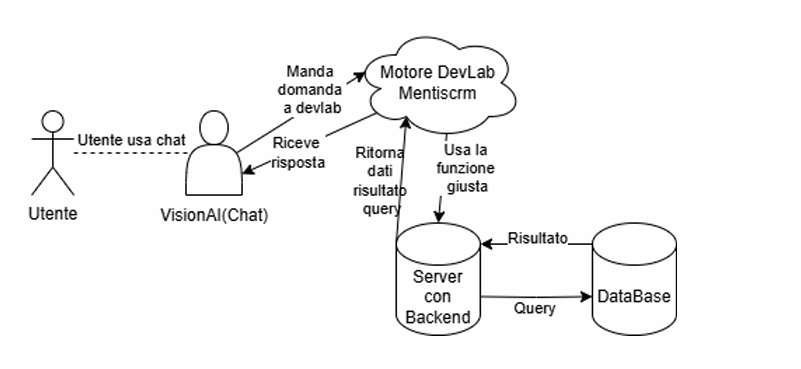
\includegraphics[width=\textwidth]{thesis/files/img/FlussoDatiVisionAI.PNG}
    \caption{Flusso operativo di VisionAI.}
    \label{fig:Architettura-generale}
\end{figure}

L'immagine \ref{fig:Architettura-generale} rappresenta il flusso di funzionamento di VisionAI, inizia con l'inserimento di una domanda in linguaggio naturale da parte dell'utente in \textit{chat}. Il motore di DevLab elabora la richiesta e utilizzando il modello GPT trova l'\mygls{API} più adatta per la richiesta,  successivamente costruisce in modo dinamico l'URL della chiamata. Il \textit{backend} elabora la richiesta, accede al \textit{database} e restituisce i dati in formato JSON. Per concludere GPT interpreta il risultato e crea una risposta in linguaggio naturale.


\subsection{Analisi dei requisiti}
L'analisi rappresenta uno dei momenti più importanti nell'ingegneria del \textit{software}, questa attività costituisce il momento in cui le idee e i bisogni vengono trasformate in specifiche operative che guideranno in seguito la fase di progettazione, sviluppo e validazione. 
L'analisi dei requisiti in particolare ha come scopo quello di identificare le funzionalità che il sistema deve offrire per rispondere alle necessità individuate dall'azienda.
Nel contesto di VisionAI questa attività è servita a individuare quali funzionalità implementare sotto forma di \mygls{API} \mygls{REST}, quali invece dovessero essere corrette e quali requisiti vadano considerati prioritari e quali invece secondari.

All'interno della seguente tabella \ref{tab:requisiti-visionai} ho riportato i requisiti individuati nel corso dell'analisi, il codice del requisito viene creato in base al seguente metodo:
\begin{center}
\textbf{R[\textit{F/O}][\textit{O/D/F}]-NN}
\end{center}

dove:
\begin{itemize}
  \item \textbf{R} indica che si tratta di un requisito;
  \item \textbf{F/O} specifica la tipologia del requisito:
    \begin{itemize}
      \item \textbf{F}: Funzionale – descrive un comportamento o una funzione del sistema;
      \item \textbf{O}: Operativo – descrive vincoli tecnici o ambientali;
    \end{itemize}
  \item \textbf{O/D/F} specifica il grado di priorità:
    \begin{itemize}
      \item \textbf{O}: Obbligatorio – deve essere implementato;
      \item \textbf{D}: Desiderabile – migliora il sistema ma non è essenziale;
      \item \textbf{F}: Facoltativo – implementabile solo in caso di tempo o risorse aggiuntive.
    \end{itemize}
  \item \textbf{NN} è un numero progressivo per identificare univocamente ogni requisito.
\end{itemize}

\begin{longtable}{|p{3cm}|p{10cm}|}
\hline
\textbf{Codice} & \textbf{Descrizione} \\
\hline
\endfirsthead

\hline
\textbf{Codice} & \textbf{Descrizione} \\
\hline
\endhead

\hline
\endfoot

\hline
\endlastfoot


RF-O-01 & L’\mygls{API} deve permettere l’inserimento di nuovi clienti o fornitori, assegnando automaticamente un codice identificativo \texttt{CodCliFor} secondo la strategia di codifica aziendale. \\
\hline
RF-O-02& Sviluppo di un’\mygls{API} per controllare lo stato di evasione (completa, parziale o assente) degli ordini clienti o fornitori . \\
\hline
RF-O-03 & Sviluppo di un’\mygls{API} per restituire il saldo aggiornato dei conti correnti aziendali per uno specifico esercizio contabile. \\
\hline
RF-O-04 & Sviluppo di un’\mygls{API} per l’elenco degli interventi tecnici previsti ma ancora da svolgere, con filtri per data, cliente, zona, tipo. \\
\hline
RF-F-05 & \mygls{API} per recuperare richieste di assistenza filtrabili per stato, cliente, tecnico e periodo. \\
\hline
RF-O-06 & Realizzazione di un’interfaccia grafica Windows (WinForms) per configurazione, connessione e avvio dell’applicazione VisionAI. \\
\hline
RF-D-07 & Copia strutturata di un documento esistente con aggiornamento automatico di quantità, date e intestazioni. \\
\hline
RF-D-08 & Generazione automatica di documenti "evasione" a partire da ordini o bolle precedenti. \\
\hline
RF-F-09 & Estensione delle \mygls{API} di manutenzione per aggregare le attività in base alla sede del cliente (destinazione). \\
\hline
RF-F-10 & Visualizzazione, inserimento e modifica di informazioni anagrafiche dei dipendenti interni o collegati a clienti/fornitori. \\
\hline
RF-O-11 & Rendere disponibile la funzione di ricerca in rete di dati da parte dell'assistente. \\
\hline
RF-O-12 &Le \mygls{API} POST devono popolare correttamente i campi dati di \texttt{TimeIns} e \texttt{UserIns} \\
\hline
RF-O-13 & Miglioramento delle operazioni GET e POST sulla tabella \texttt{CliFor} per la corretta assegnazione dei campi \texttt{CodPdcPatr} e \texttt{CodPagam}, distinguendo tra Cliente e Fornitore. \\
\hline
RO-O-13 & Garantire a tutte le \mygls{API} sviluppate una corretta descrizione specificando l'intento dell'\mygls{API} e la struttura della chiamata per il corretto funzionamento. \\
\hline
\caption{Tabella del tracciamento dei requisiti.}
\label{tab:requisiti-visionai}
\end{longtable}



\subsection{Progettazione}
La progettazione del sistema ha rappresentato una fase cruciale per garantire coerenza con la struttura esistente, in quanto, subentrando in un progetto già avviato è stato necessario svolgere un analisi dell'architettura esistente, capendo le logiche interne per poi sviluppare nuove componenti coerenti a i vincoli strutturali.

\textbf{Struttura a livelli e \textit{pattern}} \\
L'architettura delle \mygls{API} del sistema VisionAI si basa su un modello a strati, visualizzabile nell'immagine \ref{fig:iarchitettura}, progettato per separare le responsabilità funzionali e garantire modularità e scalabilità. La struttura segue un approccio ispirato ai principi della \mygls{Clean architecture} implementato tramite l'utilizzo combinato di \textit{controller} , servizi, \textit{repository} e \mygls{DTO}, un \textit{design pattern} utilizzato per trasferire dati in un applicazione \textit{software}.
Sebbene non sia una classica architettura MVC (\textit{model-view-controller}), essendo priva di componenti di visualizzazione, la struttura può essere descritta come una \textit{Controlelr-Service-Repository} con l'integrazione di \textit{model} e \mygls{DTO}, dove:
\begin{itemize}
    \item il \textit{controller} gestisce la comunicazione esterna e funge da \textit{entry point} per le richieste \mygls{HTTP} gestendo il \textit{routing};
    \item il \textit{Service}/\textit{Repository}, in questo progetto appaiono in un unica struttura, si occupa della logica applicativa e l'accesso ai dati;
    \item i \textit{Model} rappresentano le strutture dati;
    \item i \mygls{DTO} consentono il trasferimento controllato e strutturato delle informazioni.
\end{itemize}

\begin{figure}[H]
    \centering
    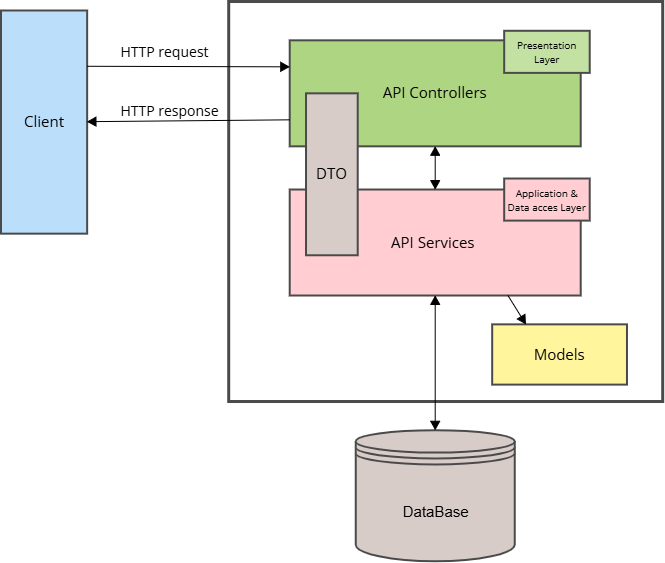
\includegraphics[width=\textwidth]{thesis/files/img/Untitled.png}
    \caption{Architettura \protect\mygls{API}.}
    \label{fig:iarchitettura}
\end{figure}


Questa architettura è stata scelta per questo tipo di struttura per vari motivi, per creare \mygls{API} \mygls{REST} facilmente interrogabili da sistemi \textit{AI}, per garantire una separazione netta delle responsabilità tra i vari livelli aiutando la manutenzione e l'estensione del sistema, proteggere i dati separando i modelli interni con oggetti esposti come i \mygls{DTO}.
Nel contesto del progetto questi sono i livelli principali:
\begin{enumerate}
    \item \textbf{\textit{Presentation layer} - \textit{Controllers}}\\
    I \textit{controller} sono collocati all'interno della cartella \texttt{Controllers} e fungono da punto di contatto tra la logica interna del sistema e l'esterno, nel caso della nostra applicazione il motore di DevLab e il \textit{chatbot}.
    Dentro l'applicazione VisionAI ogni \textit{controller} viene associato a una funzionalità o a un gruppo funzionale, come \texttt{CliForController} che gestisce l'accesso alle anagrafiche clienti/fornitori, o come \texttt{BancheController} che si occupa dell'accesso all'elaborazione dei saldi e dei conti correnti aziendali.
    Ogni \textit{controller} viene incaricato di svolgere diverse operazioni, ricevere richieste \mygls{HTTP} dal motore GPT in formato \textit{GET} o \textit{POST}, valida i parametri in ingresso controllando che siano corretti rispetto alla logica definita, inoltra la richiesta al servizio corrispondente e restituisce una risposta in formato JSON. In questo progetto non esiste una interfaccia utente, il \textit{controller} funge solo da \textit{entry point} per le richieste esterne.
    \item \textbf{\textit{Application} \& \textit{data access layer} - \textit{Services} / \textit{Repository}}\\
    Nel progetto VisionAI la logica applicativa e il \textit{data acces layer} sono stati accorpati in un unica struttura contenuta nella cartella \texttt{Services}, in cui ogni \textit{file} è dedicato in un contesto funzionale differente. Questo approccio ci fa uscire dagli \textit{standard} di un \textit{design pattern} classico, andando a creare una struttura ibrida orientata alla praticità e alla velocità di sviluppo. 
    Ciascun \textit{file} \textit{Repository}, questo il nome dei \textit{file} contenuti nella cartella, ad esempio \texttt{CliForRepository} contiene sia metodi che si occupano della \textit{businnes logic} specifica del dominio (implementazione di parametri e filtri), sia dell'interazione diretta con il \textit{database} utilizzando LINQ o Drapper.
    Come già detto ogni \textit{file} è focalizzato su un area specifica del contesto applicativo, questo consente di avere \textit{repository ad hoc} per ogni gruppo di \mygls{API}.
    \item \textbf{\textit{Data definition} e \textit{transfer} - \textit{Model} / \mygls{DTO}} \\
    Nel progetto VisionAI non viene definito un \textit{layer} apposito per i  \textit{model}, come accade nell'architettura MVC (\textit{Model-View-Controller}) classica. Tuttavia, i \textit{model} svolgono un ruolo essenziale all'interno del nostro sistema, servono a definire come sono strutturati i dati all'interno del \textit{database}, fornendo una rappresentazione diretta delle tabelle.
    Queste classi vengono richiamate all'interno dei \textit{services} per permettere l'interazione con i dati e comprenderne la struttura. A supporto di questa operazione è presente il \textit{file} \texttt{ApplicationDbContext} che definisce il contesto del \textit{database} contenendo le relazioni delle entità interessate, facilitando la navigazione tra le tabelle.
    Oltre a i \textit{model} il progetto utilizza anche \mygls{DTO}, non in maniera globale ma in maniera specifica in alcuni casi, non tutti gli \textit{enpoint} infatti ne fanno uso. Sono stati introdotti per i casi più articolati dove è necessario definire una struttura di risposta standardizzata, controllare l'esposizione evitando la fuoriuscita di dati sensibili e aggregare dati provenienti da tabelle diverse

    \item \textbf{\textit{Database layer}} \\
    Questo \textit{layer} rappresenta lo stato più profondo dell'architettura, in questo strato sono presenti i dati aziendali effettivi. Questi dati sono distribuiti su diversi \textit{database}, tutti in formato SQL Server e preesistenti, i \textit{database} utilizzati sono stati \texttt{VisionEsempio}, \texttt{VisionCommon} e \texttt{VisionAnt}.
    L'accesso alle basi di dati è configurabile nel sistema in modo dinamico tramite l'utilizzo del \textit{file} \texttt{appsetting.json}, il quale contiene le connessioni ai \textit{database} aziendali e i parametri ambientali personalizzabili.
    Durante l'esecuzione l'utente può modificare la connessione ai \textit{database} anche tramite l'utilizzo dell'interfaccia Windows \textit{form} sviluppata.
\end{enumerate}

La progettazione delle \mygls{API} oltre dell'infrastruttura già esistente ha dovuto tenere conto di un altra variabile molto importante, ovvero che queste \mygls{API} non vengono chiamate da un \textit{frontend} programmato per eseguire chiamate standardizzate ma da un \mygls{LLM} che effettua chiamate solamente con il contesto fornitogli da un \textit{prompt}. Questo elemento ha comportato scelte progettuali di grande impatto. Innanzitutto le \mygls{API} sono progettate per essere facilmente interpretabili dal modello mantenendo sempre parametri chiari e assenza totale di ambiguità per i nomi dei campi dati. Inoltre il contesto fornito all'\textit{AI}, in questo caso GPT-4, può essere caricato solamente tramite prompt di testo dalla dimensione limitata, questa caratteristica porta all'impossibilità di costruire \mygls{API} esageratamente complesse o con troppi campi dati per effettuare chiamate molto precise. Diventa quindi di fondamentale importanza la capacità di descrivere il funzionamento delle \mygls{API} in modo riassuntivo e specifico, per fornire il \textit{prompt} corretto e consentire al modello \mygls{LLM} di effettuare una chiamata corretta. Un altro aspetto di estrema importanza progettuale è la robustezza contro \textit{input} imprevedibili, il sistema \textit{backend} quindi deve essere robusto nel controllo degli \textit{input} nelle \mygls{API} POST, effettuando la normalizzazione dei dati, gestendo casi di dati mancanti o inadeguati e gestendo messaggi di errore o comportamenti imprevisti.


\textbf{Progettazione Windows \textit{form}}\\
Nel contesto dell'applicazione VisionAI è stato introdotto un componente accessorio riutilizzabile con l'obiettivo di centralizzare l'accesso all'applicazione in punti specifici all'interno dei prodotti dell'azienda. 
L'obiettivo del \textit{form} è centralizzare l'esecuzione dell'applicativo, infatti rappresenta il punto di ingresso per avviare l'applicazione permettendo di visualizzare e modificare in maniera semplice i dati legati al \textit{database} e alle credenziali d'accesso. Il \textit{form} è stato infatti richiesto per due motivi principali ovvero gestire in modo rapido la connessione al \textit{database} senza dover modificare stringhe a livello codice, e supportare configurazioni lanciando l'\textit{app} in modo diretto dal gestionale e permettendo all'utente di salvare i propri dati di accesso e riutilizzarli all'interno di sessioni successive.
L'utilizzo di Windows \textit{form} è stata richiesta in modo diretto dall'azienda, mantenendo un interfaccia semplice focalizzata sulla  connessione all'\textit{app} vera e propria.
Per garantire la connessione al \textit{database} viene modificato in modo diretto il \textit{file} \texttt{appsetting.json}, che contiene tutte le stringhe di connessione.
Per quanto riguarda invece la gestione delle credenziali e delle sessioni di accesso il discorso è più lungo.
Questa sezione ha l'obiettivo di mantenere la connessione alla \textit{chat} anche in caso la connessione venga interrotta a causa delle sessioni a tempo. Risulta scomodo l'inserimento delle credenziali in maniera manuale ogni trenta minuti.
Per risolvere questo problema è stato aggiunto al \textit{form} una sezione che consente l'inserimento delle credenziali iniziali, esegue la chiamata di \textit{login} e ottiene in  risposta due \textit{token} uno di accesso e uno di \textit{refresh}. Questi due \textit{token} vengono salvati in \textit{file} locali in particolare: 
\begin{itemize}
    \item \texttt{log.json}: salva il \textit{token} di accesso alla sessione che sta per essere avviata.
    \item \texttt{ses.json}: salva il \textit{token} di \textit{refresh}, utilizzato per aggiornare la sessione corrente senza il reinserimento dei dati.
    \item \texttt{data.json}: registra l'orario della generazione dei \textit{token}.
\end{itemize}
Ogni sessione ha la durata \textit{standard} di trenta minuti e per garantire quindi continuità nell'uso della \textit{chat}, viene letto il valore temporale di \texttt{data.json}, se sono trascorsi più di trenta minuti il sistema esegue automaticamente una chiamata di \textit{refresh} e sovrascrive i \textit{token} precedenti con quelli nuovi ricevuti come risposta.

\subsection{Difficoltà incontrate durante la codifica}
Lo sviluppo delle \mygls{API} per VisionAI ha richiesto un attività di codifica approfondita, caratterizzata anche dai vincoli strutturali imposti dalla base dati esistente e dall'architettura predefinita. 
Una delle complessità principali è stata la gestione dell'accesso a dati distribuiti su più tabelle relazionate. Praticamente tutte le \mygls{API} sviluppate nel periodo infatti chiedevano la risposta a domande complesse e per garantire ciò era necessario accedere a dati provenienti da entità diverse. Per affrontare queste difficoltà è stato adottato Entity Framework Core, un \mygls{ORM} che contente di eseguire \textit{query} SQL in maniera astratta tramite LINQ-to-Entities, questo approccio ha permesso di gestire le relazioni tra tabelle attraverso \textit{join} espliciti all'interno del codice ma senza usare codice SQL, applicare filtri dinamici per permettere l'utilizzo di parametri all'interno della chiamata, recuperare e proiettare i dati in strutture che poi vengono trasformate in \mygls{DTO}. È possibile visualizzare il funzionamento ad alto livello di un sistema \mygls{ORM} nella figura \ref{fig:ORM}.
Particolare attenzione è stata dedicata anche alla validazione dei dati in \textit{input} per quanto riguarda le \mygls{API} \textit{POST}, effettuando controlli sui campi obbligatori, normalizzando i dati prima dell'inserimento nel \textit{database} e aggiornando lo \textit{script} di assegnazione automatica del campo \texttt{CodCliFor} applicando l'algoritmo di assegnazione aziendale.

\begin{figure}[H]
    \centering
    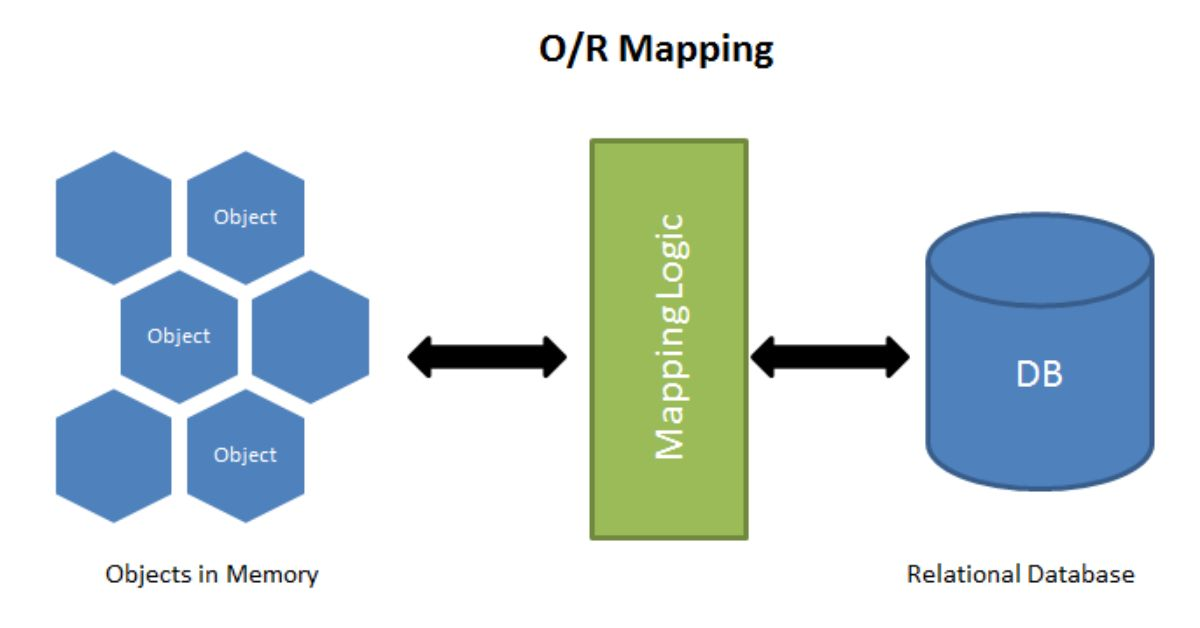
\includegraphics[width=.7\columnwidth]{thesis/files/img/ORM.jpg}
    \caption[Diagramma di funzionamento di un ORM.]{
        Diagramma di funzionamento di un ORM.\\
\textit{Fonte:\url{https://www.youstable.com/it/blog/cos'è-ORM-nella-programmazione/}}
    }
    \label{fig:ORM}
\end{figure}




\subsection{Verifica e presentazione dei risultati ottenuti}
La verifica ha rappresentato un'attività molto importante del processo di sviluppo, al fine di garantire la correttezza e coerenza delle funzionalità implementate.
Sebbene, per motivi di tempo, non siano stati introdotti \textit{test} automatici strutturati, ho condotto un'attenta validazione manuale di tutte le \mygls{API} sviluppate, sia negli ambienti locali sia nell'integrazione con il \textit{chatbot}.\\
\textbf{\textit{Test} funzionali delle \mygls{API}} \\ 
Ogni \mygls{endpoint} è stato \textit{testato} singolarmente mediante strumenti di ispezione delle \mygls{API} tra cui Swagger, utilizzato durante lo sviluppo per l'esposizione degli \textit{enpoint}, il controllo dei parametri, la correttezza delle risposte \mygls{HTTP} e la visualizzazione della documentazione interattiva delle \mygls{API}. Altro strumento utilizzato è stato Postman, impiegato per simulare chiamate reali dinamiche tramite OData, per visualizzare le risposte in formato JSON.
Per ogni \mygls{API} sviluppata è stato verificato: 
\begin{itemize}
    \item il corretto \textit{routing},
    \item la validità dei parametri e la logica a loro collegata,
    \item la coerenza delle risposte con i dati effettivamente presenti nel \textit{database},
    \item la corretta gestione degli errori,
    \item coerenza dei dati rispetto la logica richiesta.
\end{itemize}
Oltre all'integrazione di \textit{test} locali tramite gli strumenti citati, sono stati svolti \textit{test} sull'integrazione effettiva delle \mygls{API} con l'assistente utilizzando Ngrok per esporre il \textit{backend} locale rendendolo accessibile al motore esterno di DevLab.
Al termine delle attività sono state sviluppate con successo una serie di nuove \mygls{API} che integrano funzionalità e permettono all'assistente virtuale di rispondere in modo corretto a domande collegate a nuovi contesi.
Nella tabella \ref{tab:api-sviluppate} presento tutte le \mygls{API} sviluppate e sistemate.

\begin{table}[H]
\centering
\begin{tabular}{|p{5cm}|p{3cm}|p{4cm}|}
\hline
\textbf{Nome API} & \textbf{Metodo} & \textbf{Tipologia} \\
\hline
Dipendenti (Anagrafiche Dipendenti) & \textit{GET / POST} & Nuova \\
\hline
Banche (Saldi Conti Correnti) & \textit{GET} & Nuova \\
\hline
Ordini Evasi / Non Evasi & \textit{GET} & Nuova \\
\hline
Manutenzioni da Eseguire & \textit{GET} & Nuova \\
\hline
Manutenzioni per Destinazione & \textit{GET} & Nuova \\
\hline
SqlTraducer & \textit{GET} & Aggiornata \\
\hline
CliFor (Clienti/Fornitori) & \textit{GET / POST} & Aggiornata \\
\hline
Contatti (Anagrafiche Contatti) & \textit{GET / POST} & Aggiornata \\
\hline
Attivit\`a & \textit{GET / POST} & Aggiornata \\
\hline
\end{tabular}
\caption{API sviluppate e sistemate durante il periodo di stage.}
\label{tab:api-sviluppate}
\end{table}


\textbf{Windows \textit{from}}\\
Anche per il Windows \textit{form} non sono stati effettuati dei \textit{test} automatici ma abbiamo controllato le funzionalità verificando l'avvio dell'applicazione, la corretta modifica delle stringhe di connessione al \textit{database}, il salvataggio di una nuova connessione ad un nuovo \textit{database} e funzionalità collegate alla semplice interfaccia sviluppata che è possibile visualizzare nell'immagine \ref{fig:interfaccia-form}.

\begin{figure}[H]
    \centering
    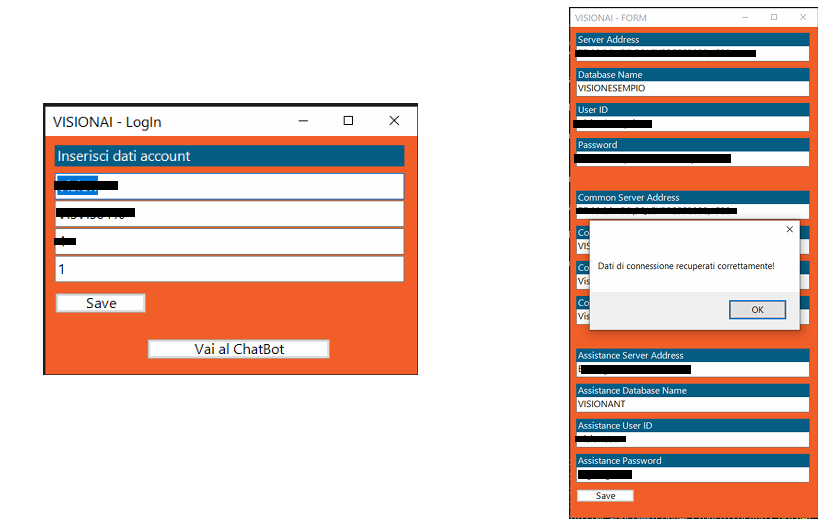
\includegraphics[width=\textwidth]{thesis/files/img/FORM-FINALE.PNG}
    \caption{Interfaccia finale \textit{form}.}
    \label{fig:interfaccia-form}
\end{figure}



\section{Sistema di assegnazione automatica per VisionAssistance}
Lo sviluppo del modulo di assegnazione automatica ha rappresentato una delle sfide più articolate e stimolanti dell'esperienza di \textit{stage}. L'obiettivo principale era quello di progettare un sistema in grado di rendere automatica l'assegnazione degli interventi ottimizzando una serie di variabili temporari, logistiche e contrattuali.
Data la complessità del dominio e l'alto numero di vincoli da rispettare si è deciso di affrontare il problema mediante la realizzazione di un \mygls{PoC},prodotto incompleto per dimostrare la fattibilità, tipo un prototipo, producendo un prodotto funzionante ma limitato.

\subsection{Analisi dei requisiti}
L'attività di definizione e raccolta dei requisiti si è basata su una stretta collaborazione con il \textit{tutor} aziendale e con il \textit{team} interno di VisioneImpresa. I requisiti sono stati definiti partendo da una serie di specifiche fornite in forma di documenti e integrate con vari incontri informali e sessioni di chiarimento con personale specializzato nel contesto di VisionAssistance. 
Alla base dei requisiti si pone l'obiettivo creare un sistema di l'assegnazione automatica dei tecnici agli interventi da svolgere, effettuando una pianificazione compatibile con diverse variabili come le disponibilità temporali dei tecnici e dei clienti, i vincoli contrattuali, le distanze fisiche, i tempi di spostamento e la priorità .

Nella tabella \ref{tab:req-agent} sono contenuti tutti i requisiti individuati, il codice viene definito nel seguente modo: 
\begin{center}
\textbf{R[\textit{O/D/F}]-NN}
\end{center}

dove:
\begin{itemize}
  \item \textbf{R} indica che si tratta di un requisito;
  \item \textbf{O/D/F} specifica il grado di priorità:
    \begin{itemize}
      \item \textbf{O}: Obbligatorio – deve essere implementato;
      \item \textbf{D}: Desiderabile – migliora il sistema ma non è essenziale;
      \item \textbf{F}: Facoltativo – implementabile solo in caso di tempo o risorse aggiuntive.
    \end{itemize}
  \item \textbf{NN} è un numero progressivo per identificare univocamente ogni requisito.
\end{itemize}

\begin{longtable}{|c|p{13.5cm}|}
\hline
\textbf{Codice} & \textbf{Descrizione} \\
\hline
RO-01 & Rispettare orari di apertura e giorni lavorativi specificati dal cliente tramite la tabella \texttt{P\_Orari}. \\
\hline
RO-02 & Considerare gli orari lavorativi settimanali dei tecnici contenuti nella tabella \texttt{CalendSett}. \\
\hline
RO-03 & Rispettare festività e orari speciali contenuti nella tabella \texttt{CalendDay}. \\
\hline
RF-04 & Utilizzare \textit{Google Places \mygls{API}} per verificare apertura delle attività. \\
\hline
RO-05 & Aggiungere tempo amministrativo fisso o in percentuale configurato per ogni intervento. \\
\hline
RO-06 & Pianificare interventi solo in presenza di sovrapposizione oraria tra cliente e tecnico. \\
\hline
RO-07 & Considerare partenza del tecnico dalla sede aziendale di appartenenza. \\
\hline
RO-08 & Mantenere orario se la data prevista è futura, ricalcolare se è già trascorsa. \\
\hline
RO-09 & Rispettare l'assegnazione del tecnico da contratto se presente. \\
\hline
RD-10 & Se il tecnico del contratto differisce da quello del buono, sostituirlo con quello corretto. \\
\hline
RD-11 & Consentire la sostituzione del tecnico solo se non vincolato da contratto. \\
\hline
RO-13 & Supportare assegnazioni spezzate per interventi di lunga durata. \\
\hline
RF-14 & Prevedere \textit{fallback} in caso di assenza di tecnici disponibili. \\
\hline
RD-15 & Generare \textit{output} in formato JSON.  \\
\hline
\caption{Tabella dei requisiti individuati per il modulo di assegnazione interventi.}
\label{tab:req-agent}
\end{longtable}

\subsection{progettazione}
Come anticipato nella sezione \ref{sec:pianificazione-attività} per motivi legati ai tempi del progetto, abbiamo deciso di dividere il lavoro, io mi sono concentrato principalmente sulla progettazione e implementazione della \textit{pipeline} dei dati.
Questa parte del progetto costituisce la base di informazioni su cui opera l'algoritmo di assegnazione automatica sviluppato in parallelo dal mio collega.
La progettazione ha seguito principi di modularità e riusabilità e disaccoppiamento delle responsabilità, come è visibile anche solo a livello di struttura della \textit{repository} nella figura \ref{fig:atruttura-pipeline} fissando come obiettivi principali:
\begin{itemize}
    \item Modularità del sistema, ogni componente svolge un compito preciso e può essere modificato indipendentemente.
    \item Automazione del flusso dei dati, la \textit{pipeline} è progettata per essere avviata con un unico comando.
    \item Standardizzazione, l'\textit{output} di questo modulo è standardizzato per essere compatibile con il sistema di assegnazione automatica.
    \item Estensibilità, la struttura modulare permette l'aggiunta di nuovi componenti in maniera semplice senza modificare la logica esistente.
\end{itemize}

\begin{figure}[H]
    \centering
    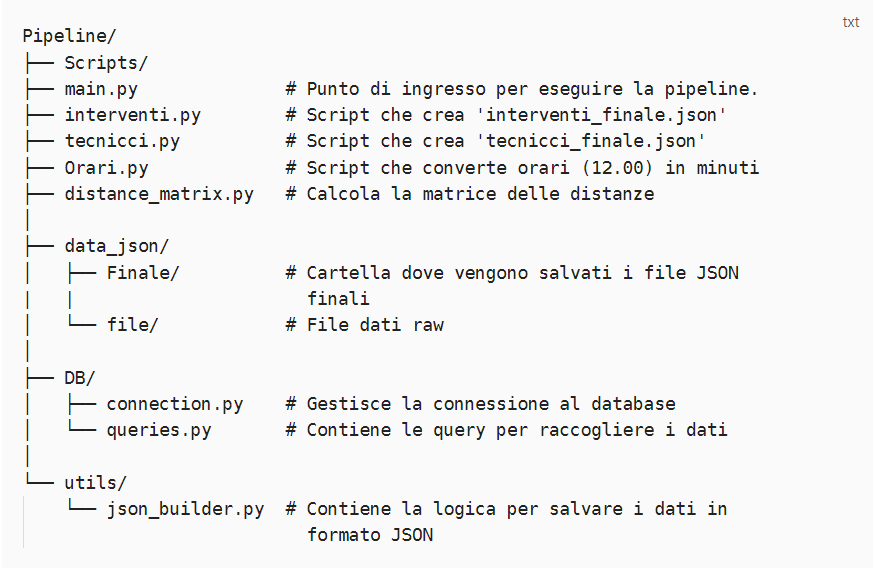
\includegraphics[width=\textwidth]{thesis/files/img/Cattura.PNG}
    \caption{Struttura delle \textit{repository} della \textit{pipeline}.}
    \label{fig:atruttura-pipeline}
\end{figure}

Dal punto di vista architetturale la \textit{pipeline} è organizzata in moduli indipendenti come si può visualizzare nella figura \ref{fig:giagram-pip}, sviluppati in Python e raggruppati in diverse cartelle come \texttt{Scripts}, \texttt{DB} e \texttt{data\_json}, ogni modulo svolge un passaggio chiave:
\begin{itemize}
    \item \texttt{Connection}: stabilisce la connessione con il \textit{database} SQL Server utilizzando SQLAlchemy e Pyodb, riunendo tutta la gestione delle variabili di accesso.
    \item \texttt{Queries}: contiene tutte le \textit{query} SQL utilizzate per estrarre tutti i dati necessari al fine di creare una base dati robusta per l'algoritmo di assegnazione.
    \item \texttt{Interventi}: modulo che si occupa di normalizzare tutti i dati relativi agli interventi da svolgere, gestendo vincoli, priorità, orari dei clienti e posizioni, andando a produrre il \textit{file} \texttt{interventi\_finale.json}.
    \item \texttt{Tecnici}: modulo che in maniera simile a quello degli interventi va a organizzare e normalizzare tutti i dati relativi ai tecnici andando a creare il \textit{file} \texttt{tecnici\_finale.json}.
    \item \texttt{Orari}: modulo che si occupa di convertire gli orari in minuti, per semplificare la manipolazione temporale nella sezione di \textit{scheduling}.
    \item \texttt{Distance\_matrix}: Modulo che si occupa di calcolare le distanze (in minuti) tra sedi e interventi utilizzando le \mygls{API} \textit{Google Maps Distance Matrix}, producendo il \textit{file} \texttt{distance\_matrix.json}.
\end{itemize}

\begin{figure}[H]
    \centering
    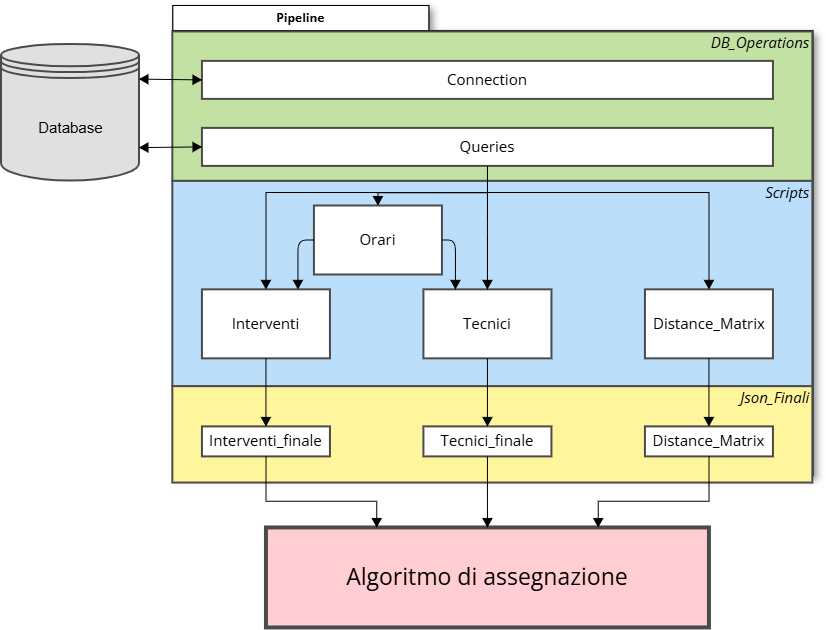
\includegraphics[width=\textwidth]{thesis/files/img/pip.png}
    \caption{Struttura architetturale della \textit{pipeline} dei dati.}
    \label{fig:giagram-pip}
\end{figure}

Nella tabella \ref{tab:scelte-chiave-agent} vengono presentate le scelte progettuali ritenute chiave.

\begin{table}[H]
\centering
\begin{tabular}{|p{4cm}|p{10cm}|}
\hline
\textbf{Decisione} & \textbf{Motivazione} \\
\hline
Linguaggio \texttt{Python} & Facilita l'integrazione, lo sviluppo rapido e l'uso di librerie avanzate per l'elaborazione dati. \\
\hline
SQLAlchemy + ODBC & Permette \textit{query} flessibili e sicure su SQL Server con gestione centralizzata delle connessioni. \\
\hline
\textit{Script} modulari & Ogni parte della \textit{pipeline} è isolata e facilmente modificabile/\textit{testabile}. \\
\hline
Gestione orari in minuti & I dati temporali sono convertiti in formato numerico per ottimizzare la gestione dei vincoli nell'algoritmo. \\
\hline
\textit{Google Distance Matrix \mygls{API}} & Calcolo realistico dei tempi di viaggio. \\
\hline
\end{tabular}
\caption{Scelte progettuali chiave adottate nella realizzazione della \textit{pipeline}.}
\label{tab:scelte-chiave-agent}

\end{table}

\subsection{Verifica e risalutati ottenuti}
La verifica per il modulo di \textit{pipeline} dei dati ha rappresentato  un'attività fondamentale per garantire la correttezza delle informazioni generate, che venendo poste alla base dell'algoritmo di decisione dei tecnici, è di estrema importanza quindi la verifica della corretta presentazione. 
Per questa sezione essendo anche un \mygls{PoC} non abbiamo introdotto sistemi di \textit{testing} automatici o semiautomatici incentrando la fase di verifica sulla validazione funzionale dei singoli script e assicurandosi che l'\textit{output} fosse coerente con i dati nel \textit{database} e integrabile con il modulo di \textit{scheduling}.

Sono stati fatti quindi \textit{test} manuali sistematici, che si concentrano sulla coerenza e la qualità dei dati prodotti. 
\begin{itemize}
    \item Controllo diretto delle \textit{query} SQL: ogni \textit{query} eseguita nel processo di estrazione dei dati è stata confrontata con i dati reali presenti nel \textit{database}, per verificarne la corrispondenza e la coerenza.
    \item Verifica dei dati aggregati: i \textit{file} JSON generati sono stati analizzati manualmente per accertare che ogni informazione fosse coerente rispetto all'origine nel \textit{database} e non ci fossero dati nulli non giustificati.
    \item Validazione del processo di trasformazione dei dati: sono state verificate le strutture dati finali per assicurare che riflettessero in maniera corretta quanto previsto in fase di progettazione
    \item Matrice delle distanze: Una attenzione maggiore è stata dedicata alla verifica della matrice dei tempi di percorrenza tra le sedi e i luoghi di intervento. Sono stati effettuati diversi \textit{test} per verificare la correttezza degli indirizzi presi in considerazione per il calcolo delle distanze, avvenuto un controllo a campione della correttezza dei tempi di viaggio restituiti, assicurare la funzionalità del sistema \textit{testando} la divisione in chiamate per rispettare i limiti imposti da Google e la gestione delle risposte \texttt{null}.
\end{itemize}


La \textit{pipeline} dei dati sviluppata è stata integrata nel \mygls{PoC}, questa unione ha confermato la corretta realizzazione di essa, in quanto tutti i \textit{file} JSON prodotti sono risultati compatibili con l'algoritmo di pianificazione, l'elaborazione dei dati ha portato a risultati concreti in rispetto dei vincoli imposti e l'\textit{output} dell'algoritmo ha evidenziato una risposta funzionale coerente pur essendo in uno scenario di prova.
L'intero lavoro si è tradotto quindi nella realizzazione di un prototipo funzionante concreto, che dimostra la fattibilità e la possibile integrazione futura nei prodotti aziendali. Per quanto riguarda i requisiti inizialmente individuati, i requisiti obbligatori sono stati tutti integrati assicurando che il sistema di assegnazione dei tecnici rispettasse i vincoli imposti mentre i requisiti desiderabili e facoltativi non sono stati integrati nel sistema.
\newpage